\section{Pre-procesamiento}
\subsection{Introducción}
Cualquier problema en ciencia de datos, comienza con un estudio exhaustivo de los datos proporcionados y realizar un \textbf{procesamiento} previo.
Si este paso es omitido, los algoritmos no se comportarán de forma óptima, debido a  que van a lidiar con unos datos que tendrán valores perdidos, que no estén normalizados, datos des-balanceados, irrelevantes, entre otras problemas. El objetivo de esta fase, es realizar ciertas transformaciones sobres los datos en bruto filtrando esta información para que los algoritmos no tengan que enfrentarse a estos problemas.
\subsection{Análisis exploratorio de los datos}
Para comenzar, se empezó leyendo la documentación aportada con los datos, la cual contenía los siguientes campos:
\begin{itemize}
	\item \textbf{Nombre:} Nombre de la característica.
	\item \textbf{Descripción:} Breve resumen explicando el origen de la característica o el enunciado de la pregunta en la encuesta.
	\item \textbf{Valores:} Tipo y/o rango que toma la característica.
\end{itemize}

Esta información es muy útil, ya que aparte de darnos un poco más de conocimiento del objetivo que queremos alcanzar con estos datos, nos da información de algunas características redundantes.

\begin{table}[!htbp]
	\begin{tabular}{|l|l|l|}
		\cline{1-3}
		CF9  &	Normalmente es posible reducir...&	Respuesta: Verdadera/Falsa. \\ \cline{1-3}
		QF9	& Variable creada a partir de CF9.  & Valor 1 si la respuesta es correcta, 0 si no. \\ \cline{1-3}
	\end{tabular}
	\label{tab:columnas_iguales}
	\caption{Comparación de dos características redundantes.}
\end{table}

Como podemos ver, estas dos columnas contienen información redundante, ya que siendo una respuesta de tipo verdadero o falso, tenemos dos columnas con la misma información. Este caso se repite en varios casos, y en todos ellos se ha optado por dejar unicamente la que tiene los valores numéricos.\\
\linebreak
El siguiente paso ha sido el de obtener las columnas que se van a usar como predictores.
La peculiaridad de este conjunto de datos tenemos 7 columnas que van a ser las que los algoritmos tienen que intentar predecir. De estas 7 columnas tenemos 6 de ellas que son de tipo ordinal, almacenando la opinión (en escala Likert) que ha tenido el entrevistado sobre la pregunta en concreto. La ultima de estas columnas es la media de las 6 columnas.\\
 A continuación se muestra una tabla con la ocurrencia de cada valor para las columnas que vamos a usar:\\
\linebreak
 \begin{figure}[!htbp]
 	 \centering
	 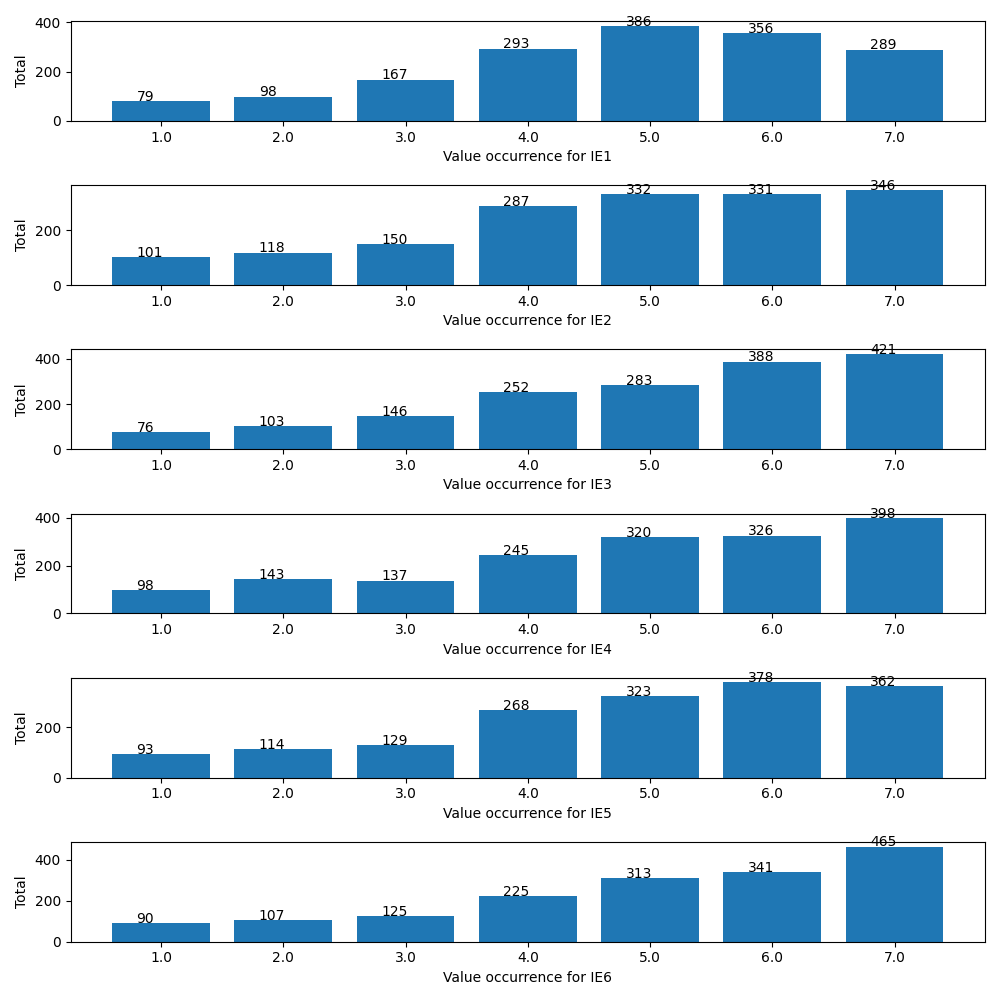
\includegraphics[scale=0.5]{src/value_occurrences.png}
	\caption{Conteo de valores para las columnas usadas como predictores}
	\label{tab:ocurrencia_valores}
\end{figure}
\linebreak
Una vez leída esta documentación y detectados algunos casos de columnas con información redundante, se cargaron los datos y se sacaron una serie de métricas. Estamos ante un conjunto de datos formados por un total de 1672 ejemplos y con 246 características (antes de realizar cualquier tipo de procesamiento), las cuales pueden ser de tipo entero, flotante o categóricas.
\pagebreak
\subsection{Pre-procesado de datos}
En este paso también se han borrado aquellas columnas las cuales corresponden a respuestas de tipo abierta. Estas características pueden llegar a contener un valor único por cada uno de los ejemplos que tenemos. En un principio, van a ser descartadas, pero en fases siguientes se podría realizar un procesamiento más exhaustivo sobre dicha columna, agrupando ciertos valores y reduciendo así la complejidad. Cabe destacar que esta información no se esta perdiendo totalmente, ya que tenemos en todos los casos una nueva columna la cual contiene si la persona respondió correctamente o no a dicha pregunta. \\
\linebreak
Un caso particular que se detectó en esta fase, fue el de las características \textbf{BFx} y \textbf{BFxAdaptada} (hay un total de 4 columnas de este tipo). Las primeras columnas de este tipo, solo contenían la respuesta las personas que realizaron la entrevista en un único año, mientras que las columnas del segundo tipo contenían la respuestas de los dos años. Antes de eliminar las columnas del primer tipo, se realizo una comprobación para ver si realmente los datos comunes entre las dos columnas eran los mismos para así asegurar que no se están perdiendo datos.
\linebreak
El siguiente paso, ha sido analizar los valores únicos de cada variable, esto nos permitió detectar valores no validos. Se encontró los siguientes casos de valores nó validos:
\begin{itemize}
	\item \textbf{Valores perdidos especificados como espacios:} Si no procesamos estos valores, el algoritmo puede detectarlo como un valor válido, introduciendo así ruido en el modelo. Estos valores se cambiaron por \textit{NaN}.
	\item \textbf{Valores perdidos especificados como "\textit{No contesta}":} Estos valores se ven sobre todo en columnas con datos ordinales. El enfoque que se ha escogido ha sido el de cambiarlas por \textit{NaN}.
	\item \textbf{Valores inválidos en la columna "\textit{género}":} Según la documentación, los únicos valores que forman esta columna son \textit{hombre} y \textit{mujer}, pero dentro del conjunto de datos se detectan valores como \textit{si} y \textit{no}. No podemos saber si la persona que contestó la encuesta se equivocó ó le llegó una versión distinta de la encuesta, así que, estos valores dentro de la columna \textit{género} se reemplazaron por \textit{NaN}.
	\item \textbf{Valores binarios codificados como strings:} Este caso no es necesariamente un valor no válido, pero se decidió cambiar estos valores binarios codificados como \textit{sí} o \textit{no} por \textit{1} y \textit{0} respectivamente. Con este cambio no vamos a perder información y vamos a ahorrarnos el codificar ciertas columnas en fases posteriores.
\end{itemize}

El siguiente paso ha sido el de obtener las columnas con una alta correlación. Hemos considerado como alta correlación, aquellas columnas cuya correlación sea mayor que 0.9\\
El resultado ha sido: \\
\begin{table}[!htbp]
	\centering
	\begin{tabular}{|l|l|l|l|}
		\cline{1-3}
		Columna 1             & Columna 2              & Correlación  \\ \cline{1-3}
		IF1.6jTiene    	      &  FI\_Insur             &  1.000000    \\ \cline{1-3}
		FinLit total(1-19)    & FinLit normaliz        & 1.000000     \\ \cline{1-3}
		ConFin(1\_7)          & ConFin(1\_8)           &  0.987110    \\ \cline{1-3}
		FinBehSinBorrow (1-6) & FinBeh con borrow(1-7) &  0.948779    \\ \cline{1-3}
	\end{tabular}
	\label{tab:correlacion}
	\caption{Matriz de correlación}
\end{table}
\linebreak
Volviendo a revisar la documentación, tenemos las siguientes descripciones:
\linebreak
\begin{itemize}
	\item \textit{FI\_Insur}: Si tiene Productos de seguro: contrato de seguros (IF1.6jTiene). Valor 1 cuando tiene alguno, en caso contrario toma valor 0.
	 \item \textit{FinLit normaliz}: Puntuación de Competencia financiera normalizada calculado dividiendo entre 19 y multiplicando por 100. Indica el porcentaje de competencia financiera general sobre 100. (columna \textit{FinLit total}).
	 \item \textit{ConFin(1\_7)}: Variable global de Conocimientos financieros generales sumando QF3 a QF9. \textit{ConFin(1\_8)} suma de QF2 a QF9.
	 \item \textit{FinBehSinBorrow (1-6)}: Suma de las variables de comportamiento financiero excepto Borrow. \textit{FinBeh con borrow(1-7) } introduce Borrow.
\end{itemize}
Como vemos, viendo la explicación de las variables, podemos prescindir de ciertas columnas. En este caso se han descartados las características de la columna 2.\\
\linebreak
Por último, se ha dividido el conjunto de datos en los conjuntos de entrenamiento y test.
\linebreak
A continuación, se va a explicar qué algoritmos se han usado para imputación de valores perdidos, codificación de características categóricas y normalización, etc. En cada subsección de \textbf{\ref{sec:algoritmos}-\nameref{sec:algoritmos}}, se especifica que algoritmos han sido aplicados a cada modelo.

\subsubsection{Valores perdidos}
Un valor perdido es aquel para el que en una variable determinada, no consta en una o más muestras de conjunto de datos. En caso de que se trabaje con un conjunto de datos con valores perdidos, se puede optar por:
\begin{itemize}
	\item \textbf{Eliminar} aquellas muestras que contengan valores perdidos.
	\item \textbf{Imputar} los valores perdidos en función de del resto de muestras.
\end{itemize}

La opción de eliminar las muestras tiene la ventaja de que no se está introduciendo información artificial al conjunto de datos, manteniendo así las características originales, pero claramente tiene una desventaja, y es que se está eliminando información, pudiendo impactar en el comportamiento de los algoritmos.\\
\linebreak
La segunda opción implica el estar modificando el conjunto de datos con muestras \textbf{artificiales}, alterando así las características del conjunto de datos pero sin eliminar información.\\
Estas muestras artificiales se pueden usar estadísticos como la \textbf{media}, \textbf{moda} de la variable con valores perdidos. El uso de estos estadísticos en esta fase tiene una gran desventaja: Solo se está usando la información de la propia variable, cabiendo la posibilidad que una o más variables del resto del conjunto de datos influyan en la variable que se está tratando. \\
\linebreak
Para evitar la desventaja del uso de estadísticos, puede usarse un algoritmo de machine learning para \textbf{predecir} que valor tendría el valor perdido de la variable que se está analizando. \\
\linebreak
Para imputar valores perdidos en una primera iteración del proceso, se ha usado el algoritmo KNN. Este algoritmo está explicado con más profundidad en la sección \textbf{\ref{alg:knn}-\nameref{alg:knn}} de este mismo documento, resumiendo, dada una muestra nueva,  este algoritmo calcula la \textbf{diferencia} entre la nueva muestra y \textbf{todas} las muestras del conjunto de datos, seleccionando la variable de salida de las $K$ muestras más cercanas y asignando el valor predicho en función de las variables de salida seleccionadas.
\subsubsection{Codificación de variables categóricas}
Existen algoritmos que no aceptan variables categóricas (Redes Neuronales, KNN, SVM, etc) por lo que un paso muy importante antes de usar estos algoritmos, es de adaptar el conjunto de datos para que el algoritmo funcione. \\
Una opción puede ser eliminar aquellas variables categóricas, pero se podría estar perdiendo información importante. Para usar estos algoritmos sin eliminar información lo más normal es \textbf{codificar} las variables categóricas.\\
Existen dos opciones para la codificación:
\begin{enumerate}
	\item \textbf{Codificación por etiqueta:} Cada valor único de la variable se sustituye por un valor entero.
	\item\textbf{Codificación \textit{one-hot }:} Se cambia la variable categórica por una serie de variables \textit{dummies}
\end{enumerate}

La codificación por etiqueta tiene la ventaja que es la más natural para los humanos y podría parecer suficiente, pero tiene una gran desventaja: Los valores enteros tienen una \textbf{relación de orden} entre cada valor. Los algoritmos de machine learning son capaces de entender esta relación de orden y perjudicar la eficacia del modelo.\\
\linebreak
La codificación \textit{one-hot}  crea una variable por cada valor único de la variable a codificar. Cada nueva variable se asocia con un valor único y tendrá el valor $1$ cuando el valor para esa muestra sea el asociado, fijando el valor a $0$ para el resto de nuevas variables. Un ejemplo sería el siguiente:\\
Dada el siguiente conjunto de datos de ejemplo:\\
\begin{table}[!htbp]
	\centering
	\begin{tabular}{|c|c|}
		\cline{1-2}
		ID    &	  Vehículo.  \\ \cline{1-2}
		0	  &   Moto       \\ \cline{1-2}
		1	  &   Camión     \\ \cline{1-2}
		2     &   Coche      \\ \cline{1-2}
		3	  &   Moto       \\ \cline{1-2}
	\end{tabular}
	\caption{Conjunto de datos de ejemplo.}
	\label{tab:conjunto_ejemplo}
\end{table}
\linebreak
Si usamos codificamos la variable \textit{vehículo} usando la etiqueta, estaríamos imponiendo una relación de orden sobre \textit{moto, camión y coche}, pudiendo "confundir" al algoritmo. Si usamos la codificación \textit{one hot}, el conjunto quedaría:

\begin{table}[!htbp]
	\centering
	\begin{tabular}{|c|c|c|c|}
		\cline{1-4}
		ID  & Vehículo\_moto & Vehículo\_camión & Vehículo\_coche. \\ \cline{1-4}
		0	& 1  			 & 0				& 0		           \\ \cline{1-4}
		1	& 0				 & 1				& 0 			   \\ \cline{1-4}
		2   & 0 			 & 0 				& 1				   \\ \cline{1-4}
		3   & 1 			 & 0 				& 0			       \\ \cline{1-4}
	\end{tabular}
	\caption{Conjunto de datos de ejemplo tras codificar}
	\label{tab:conjunto_ejemplo_cod}
\end{table}
Como se ve en la tabla \ref{tab:conjunto_ejemplo_cod}, se ha transformado la columna \textit{vehículo} en tres columnas distintas, tomando el valor 1 cuando el valor de la variable sin codificar coincide con la variable asignada para ese valor. \\
\linebreak
Este modelo tiene una desventaja clara, y es se van a crear tantas columnas como valores único tenga la variable a codificar, esto puede incrementar significativamente el tamaño del conjunto de datos, pudiendo impactar en el rendimiento de los modelos.
